% Input common header
\documentclass[xcolor=dvipsnames]{beamer}

\usecolortheme[named=Blue]{structure}
\setbeamertemplate{itemize items}[circle]

\usepackage{smartdiagram}


\author{Dr. Paul Larsen}
\date{\today}


\title{Artificial Intelligence in Practice}
\begin{document}
\maketitle


\begin{frame}
\frametitle{Good market understanding (still) trumps technology}
    \begin{center}
\smartdiagramset{
	back arrow disabled=true,
}
\smartdiagram[flow diagram:verticall]{Market,
  Data, AI}
    \end{center}
  In practice
  \begin{itemize}
    \item Do research (e.g. \href{https://en.wikipedia.org/wiki/Design\_thinking}{design thinking}, exploratory data analyses)
    \item Define actions
  \end{itemize}
\end{frame}


\begin{frame}
\frametitle{Artificial intelligence and risk: more buzzwords that matter}
\begin{itemize}
\item Agile: \href{https://agilemanifesto.org/}{agilemanifesto.org}
\item TDD: \href{https://www.oreilly.com/library/view/test-driven-development/0321146530/}{Kent Beck, {\it Test Driven Development: By Example}}
\item DevOps: \href{https://landing.google.com/sre/books/}{Google's {\it Site Reliability Engineering}}
\end{itemize}
\begin{center}
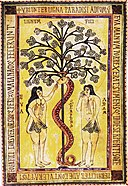
\includegraphics[height=0.35\textheight]{graphics/Codex_Aemilianensis}
\end{center}
Source: \url{https://commons.wikimedia.org/wiki/File:Codex_Aemilianensis.jpg}
\end{frame}


\begin{frame}
\frametitle{Standard Model Metrics (Almost) Never Matter}

\begin{itemize}
    \item \href{https://scikit-learn.org/stable/modules/generated/sklearn.metrics.accuracy\_score.html}{Accuracy} \cite{aletras2016predicting, echr-2}
    \item \href{https://scikit-learn.org/stable/modules/generated/sklearn.metrics.roc\_auc\_score.html\#sklearn.metrics.roc\_auc\_score}{ROC-AUC}
    \item Translation into business impact
    \item Model performance in the wild, or life is not a Kaggle competition, see also \cite{rendle2019difficulty}\newline
\end{itemize}

\begin{columns}
    \begin{column}{.3\textwidth}
\begin{figure}[ht]
    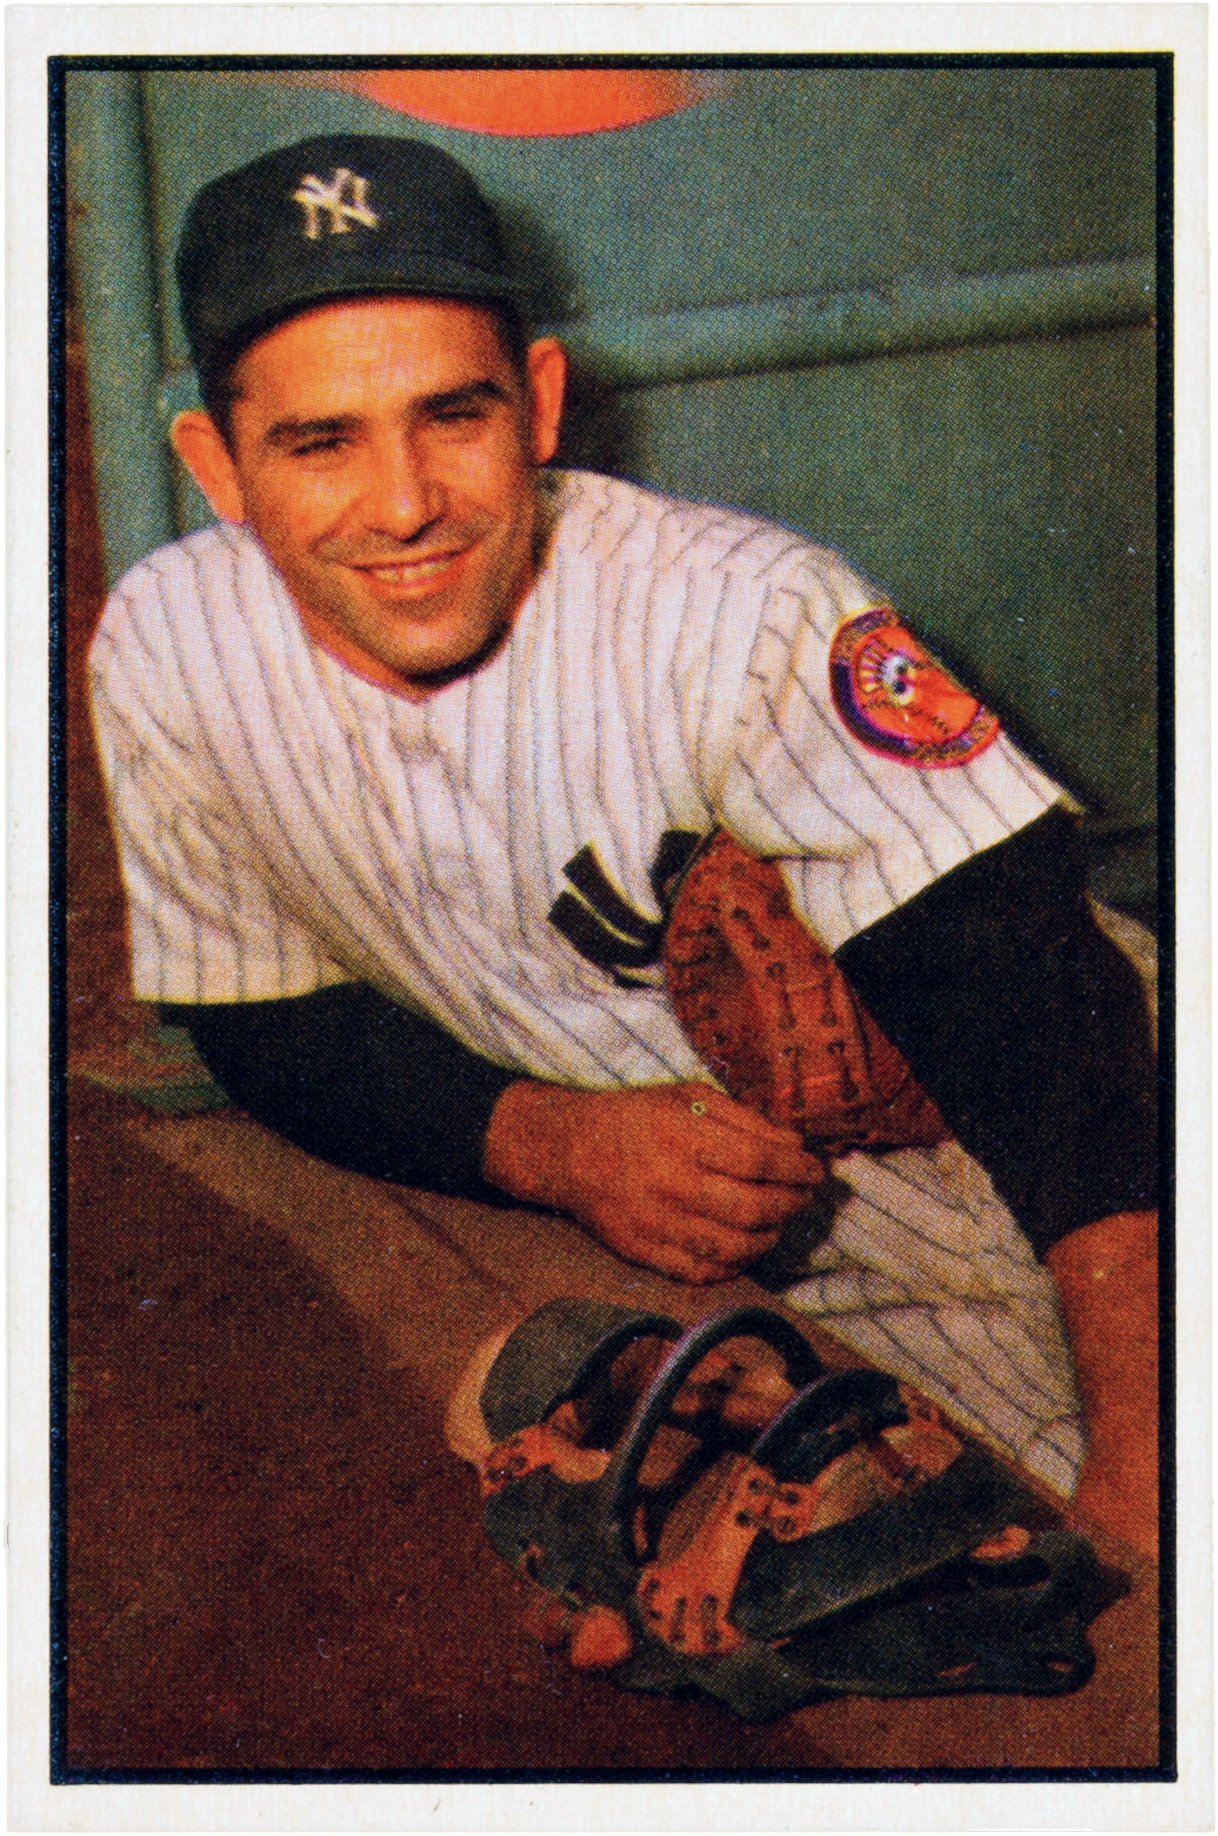
\includegraphics[height=0.4\textheight]{graphics/1953_Bowman_Yogi_Berra}
\end{figure}
\end{column}
\begin{column}{.4\textwidth}
    \emph{In theory, there is no difference between theory and practice. \newline
    In practice, there is.}\newline
    Yogi Berra
\end{column}
\begin{column}{.3\textwidth}
\end{column}
\end{columns}
\end{frame}


\begin{frame}
\frametitle{Deploying AI}

Is deploying AI different?\newline

No, since it is still is software
\begin{itemize}
\item Manage dependencies, e.g. workshop material, polytope packages
\item Library + app, e.g. \href{https://12factor.net}{12 Factor App}
\end{itemize}

Yes, since it is not standard software
\begin{itemize}
    \item Python
    \item Model maintenance
\end{itemize}
\end{frame}


\begin{frame}[allowframebreaks]
    \frametitle{References}
    \setbeamertemplate{bibliography item}[text]
    \bibliographystyle{amsalpha}
    \bibliography{../references.bib}
\end{frame}
\end{document}